


\tikzset{every picture/.style={line width=0.75pt}} %set default line width to 0.75pt        

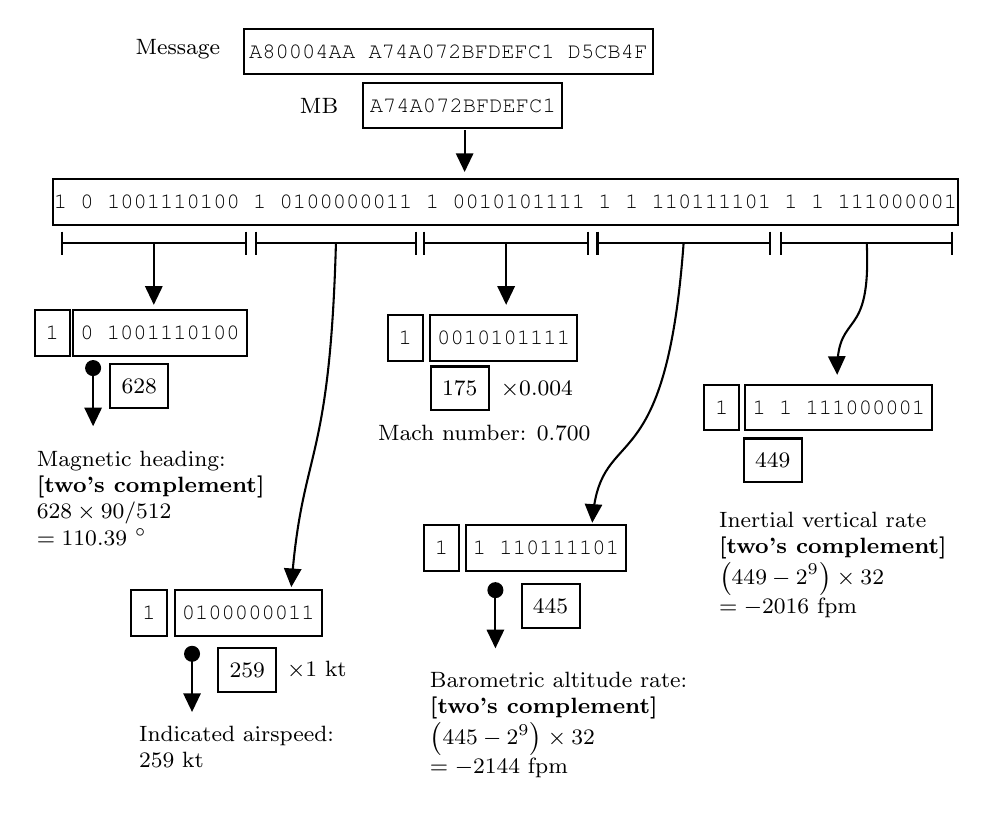
\begin{tikzpicture}[x=0.75pt,y=0.75pt,yscale=-1,xscale=1]
%uncomment if require: \path (0,574); %set diagram left start at 0, and has height of 574

%Curve Lines [id:da7633195255793686] 
\draw    (170,136.33) .. controls (166.95,244.9) and (153.77,234.23) .. (148.65,299.98) ;
\draw [shift={(148.5,302)}, rotate = 274.21] [fill={rgb, 255:red, 0; green, 0; blue, 0 }  ][line width=0.08]  [draw opacity=0] (8.93,-4.29) -- (0,0) -- (8.93,4.29) -- cycle    ;
%Curve Lines [id:da7872591125804238] 
\draw    (425.75,136.33) .. controls (427.93,184.51) and (411.85,168.16) .. (411.49,196.95) ;
\draw [shift={(411.5,199.75)}, rotate = 268.83] [fill={rgb, 255:red, 0; green, 0; blue, 0 }  ][line width=0.08]  [draw opacity=0] (8.93,-4.29) -- (0,0) -- (8.93,4.29) -- cycle    ;
%Straight Lines [id:da38985737769003403] 
\draw [line width=0.75]    (212.5,136.33) -- (291.5,136.33) ;
\draw [shift={(291.5,136.33)}, rotate = 180] [color={rgb, 255:red, 0; green, 0; blue, 0 }  ][line width=0.75]    (0,5.59) -- (0,-5.59)   ;
\draw [shift={(212.5,136.33)}, rotate = 180] [color={rgb, 255:red, 0; green, 0; blue, 0 }  ][line width=0.75]    (0,5.59) -- (0,-5.59)   ;
%Straight Lines [id:da6527595582291807] 
\draw [line width=0.75]    (131.5,136.33) -- (208.5,136.33) ;
\draw [shift={(208.5,136.33)}, rotate = 180] [color={rgb, 255:red, 0; green, 0; blue, 0 }  ][line width=0.75]    (0,5.59) -- (0,-5.59)   ;
\draw [shift={(131.5,136.33)}, rotate = 180] [color={rgb, 255:red, 0; green, 0; blue, 0 }  ][line width=0.75]    (0,5.59) -- (0,-5.59)   ;
%Straight Lines [id:da4403111582772137] 
\draw [line width=0.75]    (38,136.33) -- (126.5,136.33) ;
\draw [shift={(126.5,136.33)}, rotate = 180] [color={rgb, 255:red, 0; green, 0; blue, 0 }  ][line width=0.75]    (0,5.59) -- (0,-5.59)   ;
\draw [shift={(38,136.33)}, rotate = 180] [color={rgb, 255:red, 0; green, 0; blue, 0 }  ][line width=0.75]    (0,5.59) -- (0,-5.59)   ;
%Straight Lines [id:da848356492146114] 
\draw [line width=0.75]    (296,136.33) -- (379,136.33) ;
\draw [shift={(379,136.33)}, rotate = 180] [color={rgb, 255:red, 0; green, 0; blue, 0 }  ][line width=0.75]    (0,5.59) -- (0,-5.59)   ;
\draw [shift={(296,136.33)}, rotate = 180] [color={rgb, 255:red, 0; green, 0; blue, 0 }  ][line width=0.75]    (0,5.59) -- (0,-5.59)   ;
%Straight Lines [id:da4828725839179395] 
\draw [line width=0.75]    (384.5,136.33) -- (467,136.33) ;
\draw [shift={(467,136.33)}, rotate = 180] [color={rgb, 255:red, 0; green, 0; blue, 0 }  ][line width=0.75]    (0,5.59) -- (0,-5.59)   ;
\draw [shift={(384.5,136.33)}, rotate = 180] [color={rgb, 255:red, 0; green, 0; blue, 0 }  ][line width=0.75]    (0,5.59) -- (0,-5.59)   ;
%Curve Lines [id:da9935038522352801] 
\draw    (337.5,136.33) .. controls (328.84,254.59) and (298.1,221.74) .. (293.73,268.06) ;
\draw [shift={(293.5,271)}, rotate = 273.76] [fill={rgb, 255:red, 0; green, 0; blue, 0 }  ][line width=0.08]  [draw opacity=0] (8.93,-4.29) -- (0,0) -- (8.93,4.29) -- cycle    ;
%Straight Lines [id:da9138763454834808] 
\draw    (232,82) -- (232,99) ;
\draw [shift={(232,102)}, rotate = 270] [fill={rgb, 255:red, 0; green, 0; blue, 0 }  ][line width=0.08]  [draw opacity=0] (8.93,-4.29) -- (0,0) -- (8.93,4.29) -- cycle    ;
%Straight Lines [id:da5719167617146503] 
\draw    (53,196.5) -- (53,221.5) ;
\draw [shift={(53,224.5)}, rotate = 270] [fill={rgb, 255:red, 0; green, 0; blue, 0 }  ][line width=0.08]  [draw opacity=0] (8.93,-4.29) -- (0,0) -- (8.93,4.29) -- cycle    ;
\draw [shift={(53,196.5)}, rotate = 90] [color={rgb, 255:red, 0; green, 0; blue, 0 }  ][fill={rgb, 255:red, 0; green, 0; blue, 0 }  ][line width=0.75]      (0, 0) circle [x radius= 3.35, y radius= 3.35]   ;
%Straight Lines [id:da8586327584153641] 
\draw    (100.67,334.17) -- (100.67,359.17) ;
\draw [shift={(100.67,362.17)}, rotate = 270] [fill={rgb, 255:red, 0; green, 0; blue, 0 }  ][line width=0.08]  [draw opacity=0] (8.93,-4.29) -- (0,0) -- (8.93,4.29) -- cycle    ;
\draw [shift={(100.67,334.17)}, rotate = 90] [color={rgb, 255:red, 0; green, 0; blue, 0 }  ][fill={rgb, 255:red, 0; green, 0; blue, 0 }  ][line width=0.75]      (0, 0) circle [x radius= 3.35, y radius= 3.35]   ;
%Straight Lines [id:da5437882852637099] 
\draw    (246.83,303.5) -- (246.83,328.5) ;
\draw [shift={(246.83,331.5)}, rotate = 270] [fill={rgb, 255:red, 0; green, 0; blue, 0 }  ][line width=0.08]  [draw opacity=0] (8.93,-4.29) -- (0,0) -- (8.93,4.29) -- cycle    ;
\draw [shift={(246.83,303.5)}, rotate = 90] [color={rgb, 255:red, 0; green, 0; blue, 0 }  ][fill={rgb, 255:red, 0; green, 0; blue, 0 }  ][line width=0.75]      (0, 0) circle [x radius= 3.35, y radius= 3.35]   ;
%Straight Lines [id:da25498702942309937] 
\draw    (252,136.33) -- (252,163) ;
\draw [shift={(252,166)}, rotate = 270] [fill={rgb, 255:red, 0; green, 0; blue, 0 }  ][line width=0.08]  [draw opacity=0] (8.93,-4.29) -- (0,0) -- (8.93,4.29) -- cycle    ;
%Straight Lines [id:da003886423114634052] 
\draw    (82.25,136.33) -- (82.25,163) ;
\draw [shift={(82.25,166)}, rotate = 270] [fill={rgb, 255:red, 0; green, 0; blue, 0 }  ][line width=0.08]  [draw opacity=0] (8.93,-4.29) -- (0,0) -- (8.93,4.29) -- cycle    ;

% Text Node
\draw    (125.63,33) -- (322.63,33) -- (322.63,55) -- (125.63,55) -- cycle  ;
\draw (224.13,44) node  [font=\footnotesize] [align=left] {{\fontfamily{pcr}\selectfont A80004AA A74A072BFDEFC1 D5CB4F}};
% Text Node
\draw (161.88,70) node  [font=\footnotesize] [align=left] {MB};
% Text Node
\draw    (33.7,105.5) -- (469.7,105.5) -- (469.7,127.5) -- (33.7,127.5) -- cycle  ;
\draw (251.7,116.5) node  [font=\footnotesize] [align=left] {{\fontfamily{pcr}\selectfont 1 0 1001110100 1 0100000011 1 0010101111 1 1 110111101 1 1 111000001}};
% Text Node
\draw    (183.13,59) -- (279.13,59) -- (279.13,81) -- (183.13,81) -- cycle  ;
\draw (231.13,70) node  [font=\footnotesize] [align=left] {{\fontfamily{pcr}\selectfont A74A072BFDEFC1}};
% Text Node
\draw    (24.88,168.5) -- (41.88,168.5) -- (41.88,190.5) -- (24.88,190.5) -- cycle  ;
\draw (33.38,179.5) node  [font=\footnotesize] [align=left] {{\fontfamily{pcr}\selectfont 1}};
% Text Node
\draw    (43.26,168.5) -- (127.26,168.5) -- (127.26,190.5) -- (43.26,190.5) -- cycle  ;
\draw (85.26,179.5) node  [font=\footnotesize] [align=left] {{\fontfamily{pcr}\selectfont 0 1001110100}};
% Text Node
\draw    (61.26,194.75) -- (89.26,194.75) -- (89.26,215.75) -- (61.26,215.75) -- cycle  ;
\draw (75.26,205.25) node  [font=\footnotesize] [align=left] {628};
% Text Node
\draw    (71.38,303.5) -- (88.38,303.5) -- (88.38,325.5) -- (71.38,325.5) -- cycle  ;
\draw (79.88,314.5) node  [font=\footnotesize] [align=left] {{\fontfamily{pcr}\selectfont 1}};
% Text Node
\draw    (92.26,303.5) -- (163.26,303.5) -- (163.26,325.5) -- (92.26,325.5) -- cycle  ;
\draw (127.76,314.5) node  [font=\footnotesize] [align=left] {{\fontfamily{pcr}\selectfont 0100000011}};
% Text Node
\draw    (113.26,331.42) -- (141.26,331.42) -- (141.26,352.42) -- (113.26,352.42) -- cycle  ;
\draw (127.26,341.92) node  [font=\footnotesize] [align=left] {259};
% Text Node
\draw    (194.88,171) -- (211.88,171) -- (211.88,193) -- (194.88,193) -- cycle  ;
\draw (203.38,182) node  [font=\footnotesize] [align=left] {{\fontfamily{pcr}\selectfont 1}};
% Text Node
\draw    (215.3,171) -- (286.3,171) -- (286.3,193) -- (215.3,193) -- cycle  ;
\draw (250.8,182) node  [font=\footnotesize] [align=left] {{\fontfamily{pcr}\selectfont 0010101111}};
% Text Node
\draw    (215.6,195.75) -- (243.6,195.75) -- (243.6,216.75) -- (215.6,216.75) -- cycle  ;
\draw (229.6,206.25) node  [font=\footnotesize] [align=left] {175};
% Text Node
\draw (248,206.75) node [anchor=west] [inner sep=0.75pt]  [font=\footnotesize] [align=left] {$\displaystyle \times 0.004$};
% Text Node
\draw (93.82,43) node  [font=\footnotesize] [align=left] {Message};
% Text Node
\draw    (347.38,204.5) -- (364.38,204.5) -- (364.38,226.5) -- (347.38,226.5) -- cycle  ;
\draw (355.88,215.5) node  [font=\footnotesize] [align=left] {{\fontfamily{pcr}\selectfont 1}};
% Text Node
\draw    (367.3,204.5) -- (457.3,204.5) -- (457.3,226.5) -- (367.3,226.5) -- cycle  ;
\draw (412.3,215.5) node  [font=\footnotesize] [align=left] {{\fontfamily{pcr}\selectfont 1 1 111000001}};
% Text Node
\draw    (212.38,272.17) -- (229.38,272.17) -- (229.38,294.17) -- (212.38,294.17) -- cycle  ;
\draw (220.88,283.17) node  [font=\footnotesize] [align=left] {{\fontfamily{pcr}\selectfont 1}};
% Text Node
\draw    (232.7,272.17) -- (309.7,272.17) -- (309.7,294.17) -- (232.7,294.17) -- cycle  ;
\draw (271.2,283.17) node  [font=\footnotesize] [align=left] {{\fontfamily{pcr}\selectfont 1 110111101}};
% Text Node
\draw (80.76,259.17) node  [font=\footnotesize] [align=left] {Magnetic heading:\\\textbf{[two's complement]}\\$\displaystyle 628\times 90/512$\\$\displaystyle =110.39\ ^{\circ }$};
% Text Node
\draw (241.42,227.67) node  [font=\footnotesize] [align=left] {Mach number: 0.700};
% Text Node
\draw (122.09,378.83) node  [font=\footnotesize] [align=left] {Indicated airspeed:\\259 kt};
% Text Node
\draw    (259.42,300.75) -- (287.42,300.75) -- (287.42,321.75) -- (259.42,321.75) -- cycle  ;
\draw (273.42,311.25) node  [font=\footnotesize] [align=left] {445};
% Text Node
\draw (277.26,368.5) node  [font=\footnotesize] [align=left] {Barometric altitude rate:\\\textbf{[two's complement]}\\$\displaystyle \left( 445-2^{9}\right) \times 32$\\$\displaystyle =-2144$ fpm};
% Text Node
\draw    (366.43,230.42) -- (394.43,230.42) -- (394.43,251.42) -- (366.43,251.42) -- cycle  ;
\draw (380.43,240.92) node  [font=\footnotesize] [align=left] {449};
% Text Node
\draw (145,341.75) node [anchor=west] [inner sep=0.75pt]  [font=\footnotesize] [align=left] {$\displaystyle \times 1$ kt};
% Text Node
\draw (409.42,291.33) node  [font=\footnotesize] [align=left] {Inertial vertical rate\\\textbf{[two's complement]}\\$\displaystyle \left( 449-2^{9}\right) \times 32$\\$\displaystyle =-2016$ fpm};


\end{tikzpicture}
